
\section{Question 1}
\begin{enumerate}[(a)]
	\item 
		\[ P(\%) = f(m, p, h_1, h_2, h_3) = 
		\frac{m}{\frac{8*2p}{3}h_1 + \frac{8*p}{6}h_2 + \frac{8*p}{6}h_3 + m)} 100\%\]
	
	\item 
		En assumant que le meme nombre de couches qui ajoutent $h_3$ reste le même qu'à la
		question a) :
		\[ P(\%) = f(m, p, h_1, h_2, h_3, h_4) = 
		\frac{m}{\frac{8*2p}{3}h_1 + \frac{8*p}{6}h_2 + \frac{8*p}{6}h_3 + \frac{8*p}{6}h_4 + m)} 100\%\]
	En assumant que le nombre de couches qui ajoutent $h_3$ est le nombre de couches restantes :  
		\[ P(\%) = f(m, p, h_1, h_2, h_3, h_4) = 
		\frac{m}{\frac{8*2p}{3}h_1 + \frac{8*p}{6}h_2 + 0h_3 + \frac{8*p}{6}h_4 + m)} 100\%\]
	\item
		\[ P(\%) = f(16000, 6, 128, 256, 0, 64) = 
		\frac{16000}{\frac{8*2*6}{3}128 + \frac{8*6}{6}256 + \frac{8*6}{6}64 + 16000)} 100\% = 70.62\%\]
\end{enumerate}


\section{Question 2}

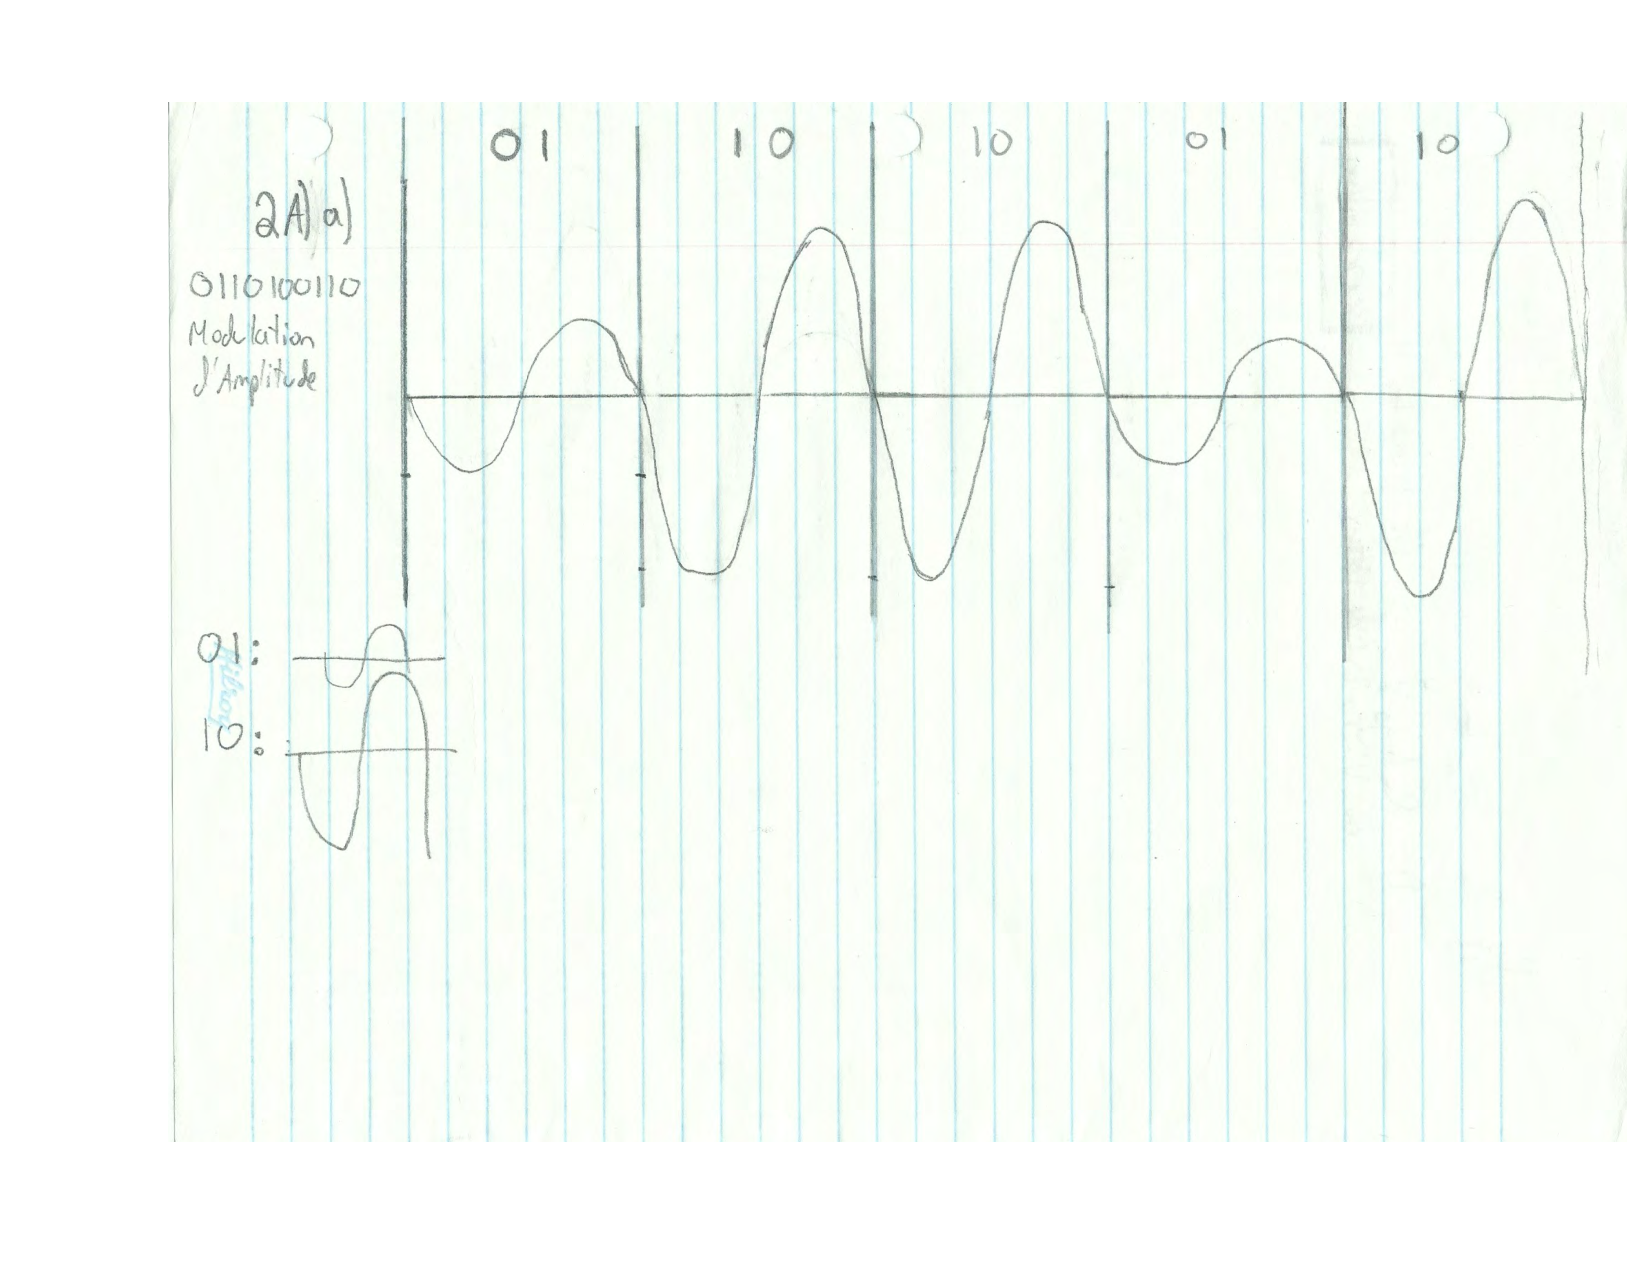
\includegraphics[scale=0.5]{julesScan}

\section{Question3}

%stuff

\section{Question 4}
\begin{enumerate}[(a)]
	\item 
		utilisation max du canal = $\frac{1000 bits}{2 * 0.250s} = 2000\frac{bits}{s}$
	\item
		$W = 2^n-1 = 2^(3bits)-1 = 7 trames$\\
		utilisation max du canal = $\frac{7 * 1000 bits}{2 * 0.250s} = 14000\frac{bits}{s}$
	\item
		$W = 2^n-1 = 2^(3bits)-1 = 7 trames$\\
		utilisation max du canal = $\frac{7 * 1000 bits}{2 * 0.250s} = 14000\frac{bits}{s}$
\end{enumerate}

% 1 mbps = 1M bits per sec
% delais 250ms
% trame 1000 bits, taille entete = 0,
% canaux codes sur 3 bits
